\subsection{Balance of Plant}
There are two main balance of plant models in the hybrid repository. The standard ideal turbine (with and without a condenser and feedwater heater) and step down turbines that allow turbine tap offtake.


\subsubsection{Simple Balance of Plant}

The balance of plant system consists of an ideal steam turbine model, a condenser, feedwater system for reheat, and a couple of valves that allow steam flow either to the turbine or as bypass to the condenser, Figure \ref{Top View SimpleBOP}. Additionally, piping exists to send condensate and rejected heat from ancillary processes directly to the condenser. The balance of plant model can handle supervisory control input for direct control of the turbine control valve and turbine bypass valve based on different sensor input. The main balance of plant system is designed to model Rankine systems.  

\begin{figure}[hbtp]
\centering
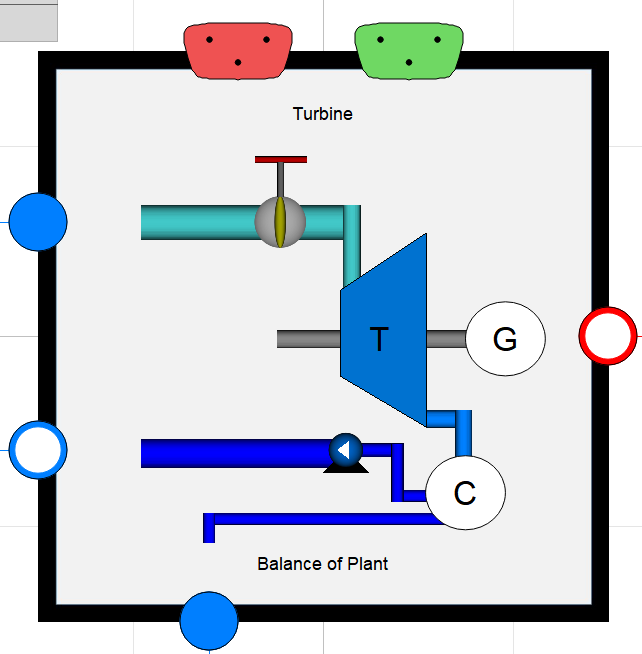
\includegraphics[scale=0.4]{pics/BOP.png}
\caption{Top Level Depiction of the Balance of Plant in the NHES package}
\label{Top View SimpleBOP}
\end{figure}


\subsubsection{Step Down Turbines}

The step-down turbines consist of a series of an ideal steam turbines connected via a singular rotational inertia shaft with bypass tap lines coming off the turbines, Figure \ref{Top View Step Down Turbines}. The purpose of this model is to allow turbine tap offtake in a dynamic system. The data record within the model includes a series of inputs that allows the user to specify the turbine tap offtake pressures. Additionally, each individual offtake fraction can be input from the data record. The outlet of the stepdown turbines does not include a condenser; therefore, a condenser model would need to be included in a separate system model if the fluid is to be re-introduced into an overall system model.
 
\begin{figure}[hbtp]
\centering
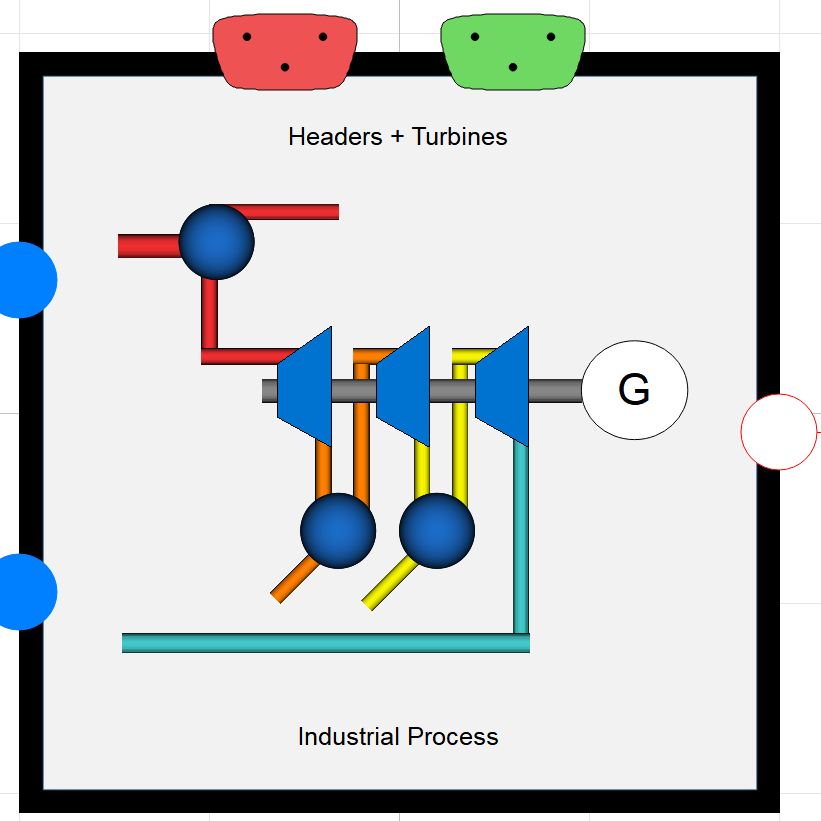
\includegraphics[scale=0.3]{pics/HeaderStepdownturbines.png}
\caption{Top Level Depiction of the StepDown Turbines in the NHES package}
\label{Top View Step Down Turbines}
\end{figure}


\subsubsection{Stage by Stage Turbine}
The stage by stage turbine package is designed to allow for detailed design of a Rankine cycle: including all turbine taps, moisture separators, reheaters, fluid junctions, and peaking capabilities. The model uses geometric design rather than system design (pressure ratios, setpoints, efficiencies). The primary design values are cross sectional and design flow deflection angles. Pressure, mass flow rate, and entropic efficiency are all uncontrolled and unspecified. 


\begin{figure}[hbtp]
\centering
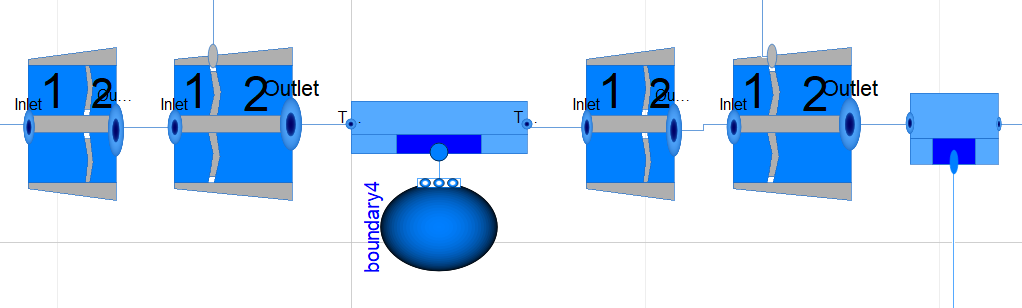
\includegraphics[scale=0.75]{pics/StagebyStageTurbine.png}
\caption{Top Level Stage by Stage Turbine Section With Stators, Rotors, a Tap, and a Moisture Separator}
\label{TVSbST}
\end{figure}


There are 8 primary components used to develop a full stage by stage turbine system. Multiple are shown in Figure \ref{TVSbST}. The first are the turbine inlet and turbine outlet components which allow for transition between 1D axial fluid components and 3D velocity cylindrical fluid flow components. The next components are the stator and rotor stages. Stator stages deflect incoming flow to better impinge and deposit energy on rotating rotor stages. Rotor stages additionally have torque connectors to connect to a physical turbine model which is responsible for linking the rotor stage torque to the electrical generator. T-junction components setup for cylindrical flow connectors allow for overpowering a rated turbine flow. The final two components deal with removing flow from the turbine. One is a turbine tap, which sets pressures equal between stages. The other is a moisture separator that removes a specific fraction of liquid flow quality. 

The stage by stage turbine has been tested from 50-100 percent steam flow. 


% content


%\subsection{Cloning the Hybrid Repository}
\label{sec:clone raven}

The first step in installing the package is to clone the HYBRID repository. To do this, use
\begin{lstlisting}[language=bash]
git clone https://github.com/idaholab/HYBRID.git
\end{lstlisting}
This will download the repository into a folder called 'hybrid'. To go inside the folder, use
\begin{lstlisting}[language=bash]
cd hybrid
\end{lstlisting}


\subsubsection{Install RAVEN and its plugins as a sub-module}

The next step is to download and install RAVEN and the submodule (e.g. TEAL, HERON) plugins as a sub-module of the HYBRID repository. 

A submodule allows you to keep another Git repository in a subdirectory of your repository. The other repository has its own history, which does not interfere with the history of the current repository. This can be used to have external dependencies such as third party libraries for example.

In order to get RAVEN do the following in the hybrid folder

\begin{lstlisting}[language=bash]
git checkout devel
\end{lstlisting}

Update the Branch

\begin{lstlisting}[language=bash]
git pull
\end{lstlisting}

to add RAVEN as a submodule
\begin{lstlisting}[language=bash]
git submodule update --init --recursive
\end{lstlisting}

\textbf{Install and Compile RAVEN. }
Once you have downloaded RAVEN as a sub-module, you have to install it. go to the \href{https://github.com/idaholab/raven/wiki/intallationMain}{RAVEN Wiki} for information about how to install it. Run all the tests outlined in the RAVEN wiki. 

\subsubsection{Inform the Framework Paths}

In order to set up the hybrid repository, you must inform the framework about the location of the Dymola python interface. For doing so, navigate to the hybrid directory:

to add RAVEN as a submodule
\begin{lstlisting}[language=bash]
cd <path to your hybrid repository>/hybrid
\end{lstlisting}
Run the following command:
\begin{lstlisting}[language=bash]
./scripts/write_hybridrc.py -p DYMOLA_PATH
\end{lstlisting}

Where DYMOLAPATH is the path to the python interface egg folder in the DYMOLA installation locally. For example:
 
\begin{lstlisting}[language=bash]
./scripts/write_hybridrc.py -p 
	"/c/Program\ Files/Dymola\ 2020x/Modelica/Library/
	python_interface/dymola.egg"
\end{lstlisting}

